\documentclass{article}
\usepackage{graphicx}
\usepackage[spanish]{babel}
\usepackage{caption}
\usepackage[style=numeric, backend=biber]{biblatex}
\addbibresource{Practica03-Documento-LaTeX-Carrillo_Bonilla.bib}
\title{El borrado histórico de las mujeres y sus consecuencias han sido un desastre para la computación.}
\author{Hugo Tonatiuh Carrillo Bonilla}
\date{24 de Septiembre de 2026}
\begin{document}
\maketitle
\section*{Introducción}
	Si uno abre la definición actual de la palabra \textit{computadora} en el diccionario de la RAE \autocite{rae}, cualquiera podría pensar que, desde siempre la palabra ha tenido un tinte exclusivamente mecánico. Resultaría muy antinatural, por supuesto, abrir el libro de Madame Bovàry y descubrir que su hermana menor es también una computadora. Esto es porque, en el principio de los tiempos, una computadora era una persona que, asistida de un ábaco y papel, se dedicaba profesionalmente y de tiempo completo a realizar operaciones aritméticas y lógicas. La razón por la que la palabra computadora y calculadora se escriben en femenino, es porque históricamente esta era una ocupación casi exclusivamente realizada por mujeres.

	Este ensayo discute varias cosas, entre ellas:
	\begin{itemize}
		\item Cómo las mujeres fueron eliminadas y excluidas de la historia de las ciencias de la computación.
		\item Las consecuencias que esto tiene, entre ellas el que la tecnología y la computación se hayan vuelto una herramienta de poder político para sectores reaccionarios y antidemocráticos.
		\item Cómo la comunidad trans, con una sobrerreprentación abrumadora en las ciencias de la computación, abre nuevos horizontes para hacer la tecnología más incluyente, universal y amigable.
	\end{itemize}
\section*{Compilador y la bruja}
	Con el advenimiento maasivo de las computadoras mecánicas en los sesenta, las antiguas computadoras --- humanas --- fueron desplazadas de un espacio que siempre había sido suyo. Históricamente, el trabajo de la computación, considerado mecánico y trivial por hombres como Euler y Gauss, fue delegado a las mujeres que no eran consideradas capaces de demostrar teoremas o entender conceptos abstractos. La asociación moderna del software con la esfera pública masculina tampoco se dio poco a poco, muchas personas que vendían las computadoras a las compañías utilizaban la cosificación sexual de las mujeres para que las tecnologías nuevas resultaran menos intimidantes para los gerentes. \cite{guardian}

	En la década de 1960, casi el 80\% de las programadoras de computadoras eran mujeres, \textbf{tan solo veinte años después}, esta cifra se redujo a tan solo el 20\% \cite{takeover}. Esta reducción de las mujeres estuvo enmarcada en una contrareacción a los avances del feminismo radical de la década de los cincuentas y sesentas, pero también estuvo profundamente influenciada por la profesionalización de este campo.
\section*{The handtyped tale.}
	En 1997, Philip Agre publicó el libro \textit{Computation and human experience}. Un libro seminal en la sociología del internet, pues argumentaba que, de forma similar a cómo la máquina del vapor transformó radicalmente las relaciones sociales al ser activamente una herramienta sociológica. Así también las computadoras, robots y autómatas de cara al Siglo XXI estaban siendo moldeadas de manera intencional por personas que se encontraban profundamente enajenadas de su realidad para sí. Notó, de forma bastante premonitoria con la información que tenemos hoy en día, que la exclusión sistemática de personas del sur global y fuera de la academia creaba un ambiente profundamente autoritario.

	Veinte años despueś, Google se deshizo de su famoso Slogan: \textit{Don't be evil} \footnote{Técnicamente no se deshicieron de él, solo dejó de ser el slogan principal del código de conducta y pasó a ser uno de muchos lineamientos.}. Que si bien fue sorprendente para observadores externos, encaja perfectamente en el modelo de Philip Agre de exclusión social sistematizada de forma tecnológica. A partir de 2021, la acumulación cualitativa de estos cambios de actitudes en el mundo de la tecnología se empezaron a hacer evidentes, y tal vez su epítome más clara fue con la fundación y propagación de la compañía \emph{Flock}.
\section*{Recordando el deseo}
	Sin embargo, de la misma manera en la que existen procesos sociológicos que hacen que Google excluya el bienestar social de su código de conducta, existen influencias que nos empujan en direcciones más esperanzadoras, pues, después de todo, fue del mismo Google de donde nació la iniciativa de codificar todo logograma escrito por la humanidad en el protocolo de \texttt{UTF-8}. Para visualizar de manera más clara estas influencias y saber cómo hacer uso de sus profundas capacidades, tal vez convenga echar un vistazo a la comunidad trans en el mundo tecnológico.

	Que las personas trans --- y en particular las mujeres trans --- existen y habitan los espacios de la computación de forma más frecuente de lo que se esperaría estadísticamente no solo se demuestra en la evidencia anecdótica, sino también en datos concretos realizados por diversos empleadores de desarrolladores a lo largo del mundo \cite{whytrans}. Eso tiene ramificaciones amplias, pues las mujeres trans son más propensas a atravesar situaciones de pobreza, discapacidad y diversidad racial que el resto de la población. Tal vez, de persona en persona, recuperemos el espacio computacional, y recordemos que estamos copiando y pegando de los hombros de gigantes como Margaret Hamilton.
	\begin{figure}
		\centering
		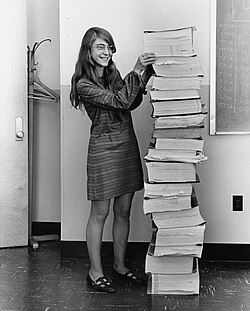
\includegraphics[width=0.2\linewidth]{./images/MargaretHamilton.jpg}
		\caption{Margaret Hamilton}
	\end{figure}
\printbibliography
\end{document}
